\chapter{LaTeX Docker \\
\small{\textit{-- JGa, JGr, CS}}
\index{LaTeXDocker} 
\index{Chapter!LaTeX Docker}
\label{Chapter::LaTeXDocker}}

In this chapter, we use a Docker container to compile a simple LaTeX document using TeX Live.

To download TeX Live and create the Dockerfile, we use the following command in our Linux terminal:

\begin{minted}{docker}
cat > Dockerfile << 'EOF'
FROM ubuntu:22.04

RUN apt-get update && apt-get install -y texlive \
    && apt-get clean && rm -rf /var/lib/apt/lists/*

WORKDIR /data

COPY sample.tex .

CMD ["pdflatex", "sample.tex"]
EOF
\end{minted}

We build and run the container as follows:

\begin{minted}{bash}
docker build -t latex-docker .
docker run --rm -v $(pwd):/data latex-docker
\end{minted}

We can finally view the sample.pdf file created from a sample LaTeX document: 
\begin{figure}[h]
  \centering
  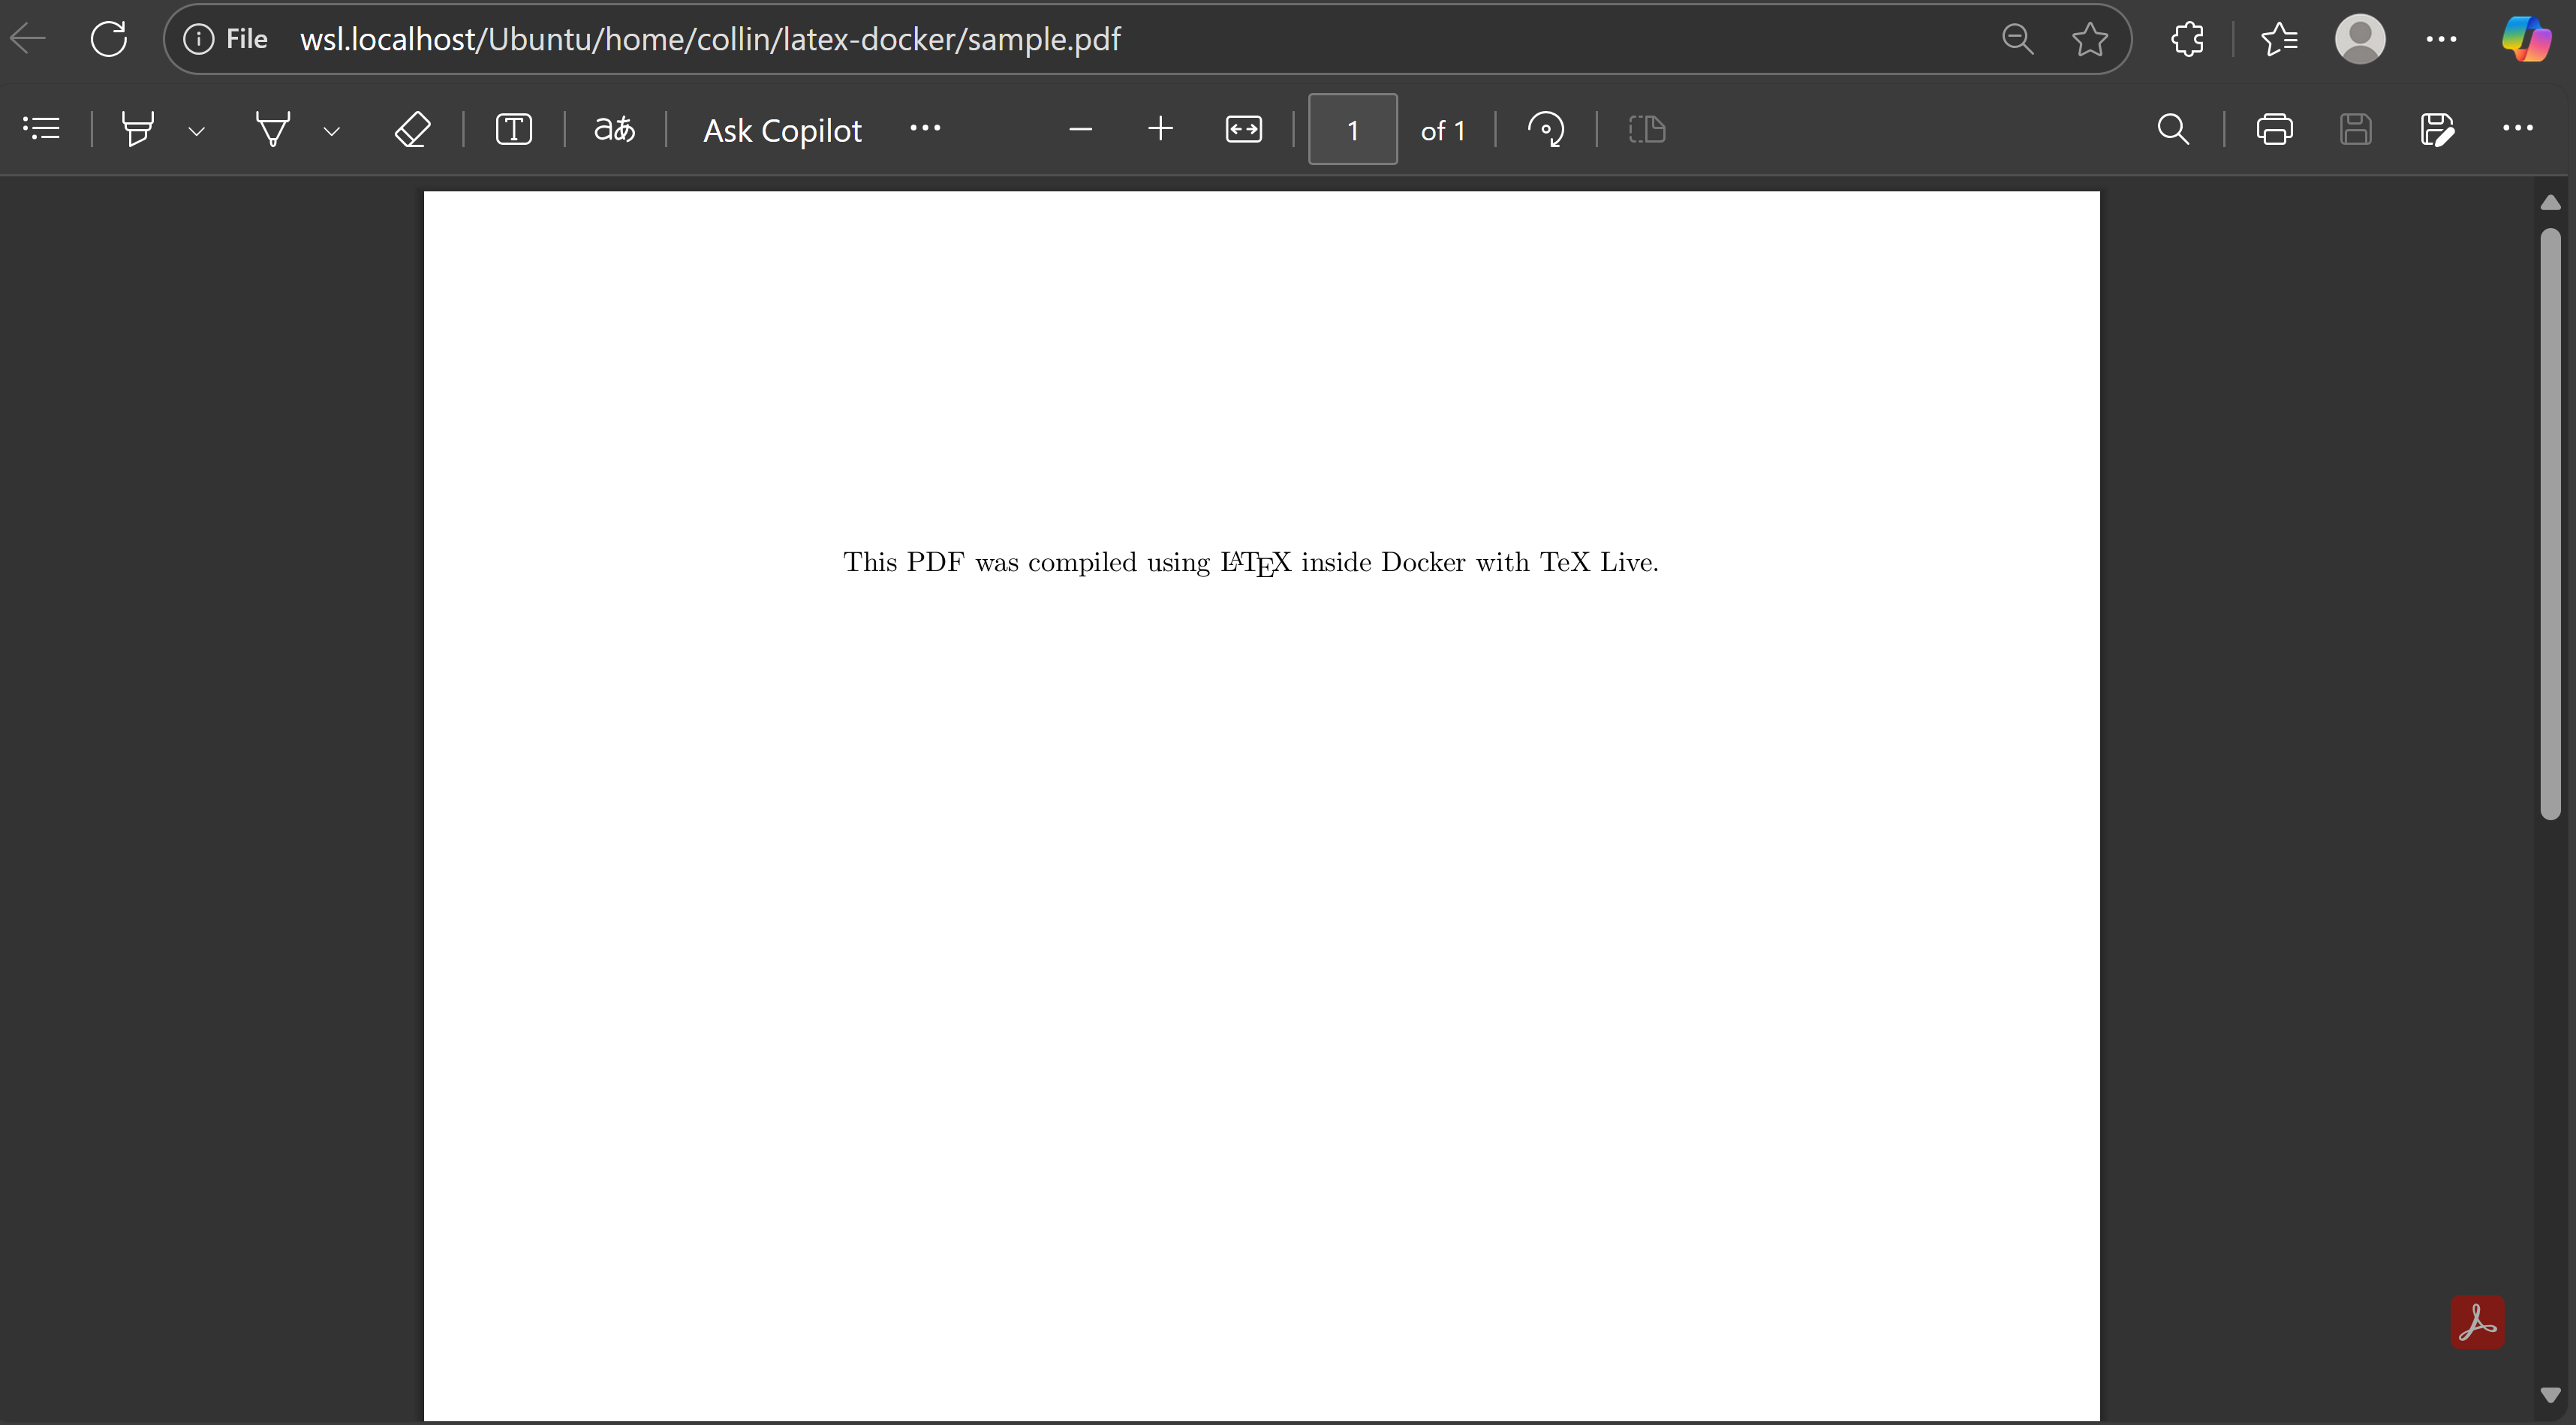
\includegraphics[width=0.7\textwidth]{png/sample_pdf_screenshot.png}
  \caption{Sample LaTeX PDF generated through Docker and TeX Live.}
  \label{fig:sample_pdf}
\end{figure}
